\chapter{Mixture models and the EM algorithm}
\label{chap:EM-algorithm}


\section{Latent variable models}
In Chapter \ref{chap:DGM} we showed how graphical models can be used to define high-dimensional joint probability distributions. The basic idea is to model dependence between two variables by adding an edge between them in the graph. (Technically the graph represents conditional
independence, but you get the point.)

An alternative approach is to assume that the observed variables are correlated because they arise from a hidden common “cause”. Model with hidden variables are also known as \textbf{latent variable models} or \textbf{LVM}s. As we will see in this chapter, such models are harder to fit than models with no latent variables. However, they can have significant advantages, for two main reasons.
\begin{itemize}
\item{First, LVMs often have fewer parameters than models that directly represent correlation in the visible space.}
\item{Second, the hidden variables in an LVM can serve as a \textbf{bottleneck}, which computes a compressed representation of the data. This forms the basis of unsupervised learning, as we will see. Figure \ref{fig:latent-variable-model} illustrates some generic LVM structures that can be used for this purpose.}
\end{itemize}

\begin{figure}[hbtp]
\centering
    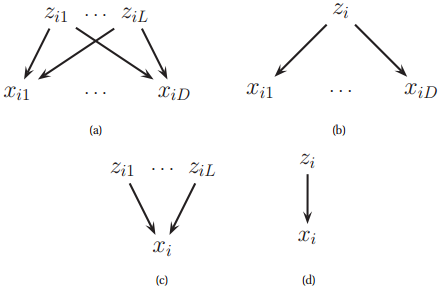
\includegraphics[scale=.60]{latent-variable-model.png}
\caption{A latent variable model represented as a DGM. (a) Many-to-many. (b) One-to-many. (c) Many-to-one. (d) One-to-one.}
\label{fig:latent-variable-model} 
\end{figure}


\section{Mixture models}
The simplest form of LVM is when $z_i \in \{1,\cdots,K\}$, representing a discrete latent state. We will use a discrete prior for this, $p(zi)=\mathrm{Cat}(\pi)$. For the likelihood, we use $p(\vec{x}_i|z_i =k)=p_k(\vec{x}_i)$, where $p_k$ is the $k$'th \textbf{base distribution} for the observations; this can be of any type. The overall model is known as a \textbf{mixture model}, since we are mixing together the $K$ base distributions as follows:
\begin{equation}
p(\vec{x}_i|\vec{\theta})=\sum\limits_{k=1}^K \pi_kp_k(\vec{x}_i|\vec{\theta})
\end{equation}

Depending on the form of the likelihood $p(\vec{x}_i|\vec{z}_i)$ and the prior $p(\vec{z}_i)$, we can generate a variety of different models, as summarized in Table \ref{tab:popular-directed-latent-variable-models}.

\begin{table}
\centering
\begin{tabular}{llll}
\hline\noalign{\smallskip}
$p(\vec{x}_i|\vec{z}_i)$ & $p(\vec{z}_i)$ & \textbf{Name} & \textbf{Section} \\
\noalign{\smallskip}\svhline\noalign{\smallskip}
MVN & Discrete & Mixture of Gaussians & 11.2.1 \\
Prod. Discrete & Discrete & Mixture of multinomials & 11.2.2 \\
\multirow{2}{*}{Prod. Gaussian} & \multirow{2}{*}{Prod. Gaussian} & Factor analysis/ & \multirow{2}{*}{12.1.5} \\
                                &                                 & probabilistic PCA&  \\
\multirow{2}{*}{Prod. Gaussian} & \multirow{2}{*}{Prod. Laplace} & Probabilistic ICA/& \multirow{2}{*}{12.6} \\
                                &                                & sparse coding     &  \\
Prod. Discrete & Prod. Gaussian & Multinomial PCA & 27.2.3 \\
\multirow{2}{*}{Prod. Discrete} & \multirow{2}{*}{Dirichlet} & Latent Dirichlet & \multirow{2}{*}{27.3}\\
                                &                            & allocation       &  \\
Prod. Noisy-OR & Prod. Bernoulli & BN20/ QMR & 10.2.3 \\
Prod. Bernoulli & Prod. Bernoulli & Sigmoid belief net & 27.7 \\
\noalign{\smallskip}\hline
\end{tabular}
\caption{Summary of some popular directed latent variable models. Here “Prod” means product, so “Prod. Discrete” in the likelihood means a factored distribution of the form $\prod_j \mathrm{Cat}(x_{ij}|\vec{z}_i)$, and “Prod. Gaussian” means a factored distribution of the form $\prod_j \mathcal{N}(x_{ij}|\vec{z}_i)$.}
\label{tab:popular-directed-latent-variable-models}
\end{table}


\subsection{Mixtures of Gaussians}
\begin{equation}
p_k(\vec{x}_i|\vec{\theta})=\mathcal{N}(\vec{x}_i|\vec{\mu}_k,\Sigma_k)
\end{equation}


\subsection{Mixtures of multinoullis}
\begin{equation}
p_k(\vec{x}_i|\vec{\theta})=\prod\limits_{j=1}^D \mathrm{Ber}(x_{ij}|\mu_{jk})=\prod\limits_{j=1}^D \mu_{jk}^{x_{ij}}(1-\mu_{jk})^{1-x_{ij}}
\end{equation}
where $\mu_{jk}$ is the probability that bit $j$ turns on in cluster $k$.

The latent variables do not have to any meaning, we might simply introduce latent variables in order to make the model more powerful. For example, one can show that the mean and covariance of the mixture distribution are given by
\begin{align}
\mathbb{E}[\vec{x}] & = \sum\limits_{k=1}^K \pi_k\vec{\mu}_k \\
\mathrm{Cov}[\vec{x}] & = \sum\limits_{k=1}^K \pi_k(\Sigma_k+\vec{\mu}_k\vec{\mu}_k^T)-\mathbb{E}[\vec{x}]\mathbb{E}[\vec{x}]^T
\end{align}
where $\Sigma_k=\mathrm{diag}(\mu_{jk}(1-\mu_{jk}))$. So although the component distributions are factorized, the joint distribution is not. Thus the mixture distribution can capture correlations between variables, unlike a single product-of-Bernoullis model.




\subsection{Using mixture models for clustering}
There are two main applications of mixture models, black-box density model(see Section 14.7.3 TODO) and clustering(see Chapter 25 TODO).

\textbf{Soft clustering}
\begin{equation}\begin{split}
r_{ik} & \triangleq p(z_i=k|\vec{x}_i,\vec{\theta})=\dfrac{p(z_i=k,\vec{x}_i|\vec{\theta})}{p(\vec{x}_i|\vec{\theta})} \\
       & =\dfrac{p(z_i=k|\vec{\theta})p(\vec{x}_i|z_i=k,\vec{\theta})}{\sum_{k'=1}^K p(z_i=k'|\vec{\theta})p(\vec{x}_i|z_i=k',\vec{\theta})}
\end{split}\end{equation}
where $r_{ik}$ is known as the \textbf{responsibility} of cluster $k$ for point $i$.

\textbf{Hard clustering}
\begin{equation}
z_i^* \triangleq \arg\max_k r_{ik}=\arg\max_k p(z_i=k|\vec{x}_i,\vec{\theta})
\end{equation}

The difference between generative classifiers and mixture models only arises at training time: in the mixture case, we never observe $z_i$, whereas with a generative classifier, we do observe $y_i$(which plays the role of $z_i$).


\subsection{Mixtures of experts}
Section 14.7.3 TODO described how to use mixture models in the context of generative classifiers. We can also use them to create discriminative models for classification and regression. For example, consider the data in Figure \ref{fig:mixture-of-experts}(a). It seems like a good model would be three different linear regression functions, each applying to a different part of the input space. We can model this by allowing the mixing weights and the mixture densities to be input-dependent:
\begin{align}
p(y_i|\vec{x}_i,z_i=k,\vec{\theta}) & =\mathcal{N}(y_i|\vec{w}_k^T\vec{x},\sigma_k^2) \\
p(z_i | \vec{x}_i,\vec{\theta}) & = \mathrm{Cat}(z_i|\mathcal{S}(\vec{V}^T\vec{x}_i))
\end{align}

See Figure \ref{fig:mixture-of-experts2}(a) for the DGM.

\begin{figure}[hbtp]
\centering
\subfloat[]{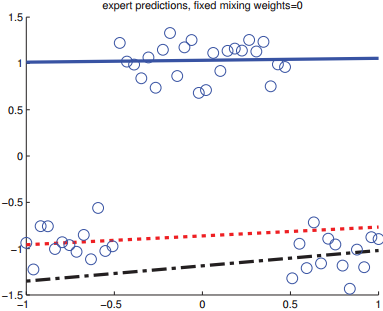
\includegraphics[scale=.60]{mixture-of-experts-a.png}} \\
\subfloat[]{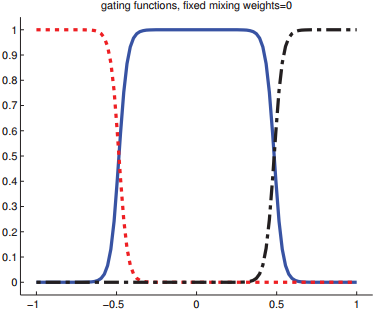
\includegraphics[scale=.60]{mixture-of-experts-b.png}} \\
\subfloat[]{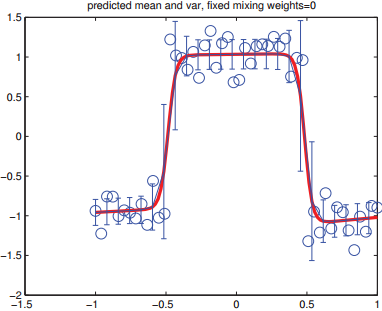
\includegraphics[scale=.60]{mixture-of-experts-c.png}}
\caption{(a) Some data fit with three separate regression lines. (b) Gating functions for three different “experts”. (c) The conditionally weighted average of the three expert predictions.}
\label{fig:mixture-of-experts} 
\end{figure}

\begin{figure}[hbtp]
\centering
    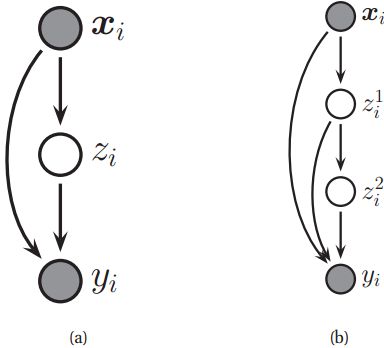
\includegraphics[scale=.50]{mixture-of-experts2.png}
\caption{(a) A mixture of experts. (b) A hierarchical mixture of experts.}
\label{fig:mixture-of-experts2} 
\end{figure}

This model is called a \textbf{mixture of experts} or MoE (Jordan and Jacobs 1994). The idea is that each submodel is considered to be an “expert” in a certain region of input space. The function $p(z_i | \vec{x}_i,\vec{\theta})$ is called a \textbf{gating function}, and decides which expert to use, depending on the input values. For example, Figure \ref{fig:mixture-of-experts}(b) shows how the three experts have “carved up” the 1d input space, Figure \ref{fig:mixture-of-experts}(a) shows the predictions of each expert individually (in this case, the experts are just linear regression models), and Figure \ref{fig:mixture-of-experts}(c) shows the overall prediction of the model, obtained using
\begin{equation}
p(y_i|\vec{x}_i,\vec{\theta})=\sum\limits_{k=1}^K p(z_i=k | \vec{x}_i,\vec{\theta})p(y_i|\vec{x}_i,z_i=k,\vec{\theta})
\end{equation}

We discuss how to fit this model in Section TODO 11.4.3.


\section{Parameter estimation for mixture models}


\subsection{Unidentifiability}


\subsection{Computing a MAP estimate is non-convex}


\section{The EM algorithm}


\subsection{Introduction}
For many models in machine learning and statistics, computing the ML or MAP parameter estimate is easy provided we observe all the values of all the relevant random variables, i.e., if we have complete data. However, if we have missing data and/or latent variables, then computing the ML/MAP estimate becomes hard.

One approach is to use a generic gradient-based optimizer to find a local minimum of the NLL$(\vec{\theta})$. However, we often have to enforce constraints, such as the fact that covariance matrices must be positive definite, mixing weights must sum to one, etc., which can be tricky. In such cases, it is often much simpler (but not always faster) to use an algorithm called \textbf{expectation maximization},or \textbf{EM} for short (Dempster et al. 1977; Meng and van Dyk 1997; McLachlan and Krishnan 1997). This is is an efficient iterative algorithm to compute the ML or MAP estimate in the presence of missing or hidden data, often with closed-form updates at each step. Furthermore, the algorithm automatically enforce the required constraints.

See Table \ref{tab:summary-of-the-applications-of-EM} for a summary of the applications of EM in this book.

\begin{table}
\caption{Some models discussed in this book for which EM can be easily applied to find the ML/ MAP parameter estimate.}
\label{tab:summary-of-the-applications-of-EM}
\centering
\begin{tabular}{ll}
\hline\noalign{\smallskip}
\textbf{Model} & \textbf{Section} \\
\noalign{\smallskip}\svhline\noalign{\smallskip}
Mix. Gaussians & 11.4.2 \\
Mix. experts & 11.4.3 \\
Factor analysis & 12.1.5 \\
Student T & 11.4.5 \\
Probit regression & 11.4.6 \\
DGM with hidden variables & 11.4.4 \\
MVN with missing data & 11.6.1 \\
HMMs & 17.5.2 \\
Shrinkage estimates of Gaussian means & Exercise 11.13 \\
\noalign{\smallskip}\hline
\end{tabular}
\end{table}


\subsection{Basic idea}
EM exploits the fact that if the data were fully observed, then the ML/ MAP estimate would be easy to compute. In particular, each iteration of the EM algorithm consists of two processes: The E-step, and the M-step. 
\begin{itemize}
\item{In the \textbf{E-step}, the missing data are inferred given the observed data and current estimate of the model parameters. This is achieved using the conditional expectation, explaining the choice of terminology.}
\item{In the \textbf{M-step}, the likelihood function is maximized under the assumption that the missing data are known. The missing data inferred from the E-step are used in lieu of the actual missing data.}
\end{itemize}

Let $\vec{x}_i$ be the visible or observed variables in case $i$, and let $\vec{z}_i$ be the hidden or missing variables. The goal is to maximize the log likelihood of the observed data:
\begin{equation}
\ell(\vec{\theta})=\log p(\mathcal{D}|\vec{\theta})=\sum\limits_{i=1}^N \log p(\vec{x}_i|\vec{\theta})=\sum\limits_{i=1}^N \log{\sum\limits_{\vec{z}_i} p(\vec{x}_i,\vec{z}_i|\vec{\theta})}
\end{equation}

Unfortunately this is hard to optimize, since the log cannot be pushed inside the sum.

EM gets around this problem as follows. Define the \textbf{complete data log likelihood} to be
\begin{equation}
\ell_c(\vec{\theta})=\sum\limits_{i=1}^N \log p(\vec{x}_i,\vec{z}_i|\vec{\theta})
\end{equation}

This cannot be computed, since $\vec{z}_i$ is unknown. So let us define the \textbf{expected complete data log likelihood} as follows:
\begin{equation}\label{eqn:auxiliary-function}
Q(\vec{\theta},\vec{\theta}^{t-1}) \triangleq \mathbb{E}_{\vec{z}|\mathcal{D},\theta^{t-1}}\left[\ell_c(\vec{\theta})\right]=\mathbb{E}\left[\ell_c(\vec{\theta})| \mathcal{D},\theta^{t-1}\right]
\end{equation}
where $t$ is the current iteration number. $Q$ is called the \textbf{auxiliary function}(see Section \ref{sec:Derivation-of-the-Q-function} for derivation). The expectation is taken wrt the old parameters, $\vec{\theta}^{t-1}$, and the observed data $\mathcal{D}$. The goal of the E-step is to compute $Q(\vec{\theta},\vec{\theta}^{t-1})$, or rather, the parameters inside of it which the MLE(or MAP) depends on; these are known as the \textbf{expected sufficient statistics} or \textbf{ESS}. In the M-step, we optimize the $Q$ function wrt $\vec{\theta}$:
\begin{equation}
\vec{\theta}^t=\arg\max_{\vec{\theta}} Q(\vec{\theta},\vec{\theta}^{t-1})
\end{equation}

To perform MAP estimation, we modify the M-step as follows:
\begin{equation}
\vec{\theta}^t=\arg\max_{\vec{\theta}} Q(\vec{\theta},\vec{\theta}^{t-1})+\log p(\vec{\theta})
\end{equation}
The E step remains unchanged.

In summary, the EM algorithm's pseudo code is as follows

\begin{algorithm}[htbp]
    \SetKwInOut{Input}{input}\SetKwInOut{Output}{output}
    \Input{observed data $\mathcal{D}=\{\vec{x}_1,\vec{x}_2,\cdots, \vec{x}_N$\},joint distribution $P(\vec{x},\vec{z}|\vec{\theta})$}
	\Output{model's parameters $\vec{\theta}$}

	// 1. identify hidden variables $\vec{z}$, write out the log likelihood function $\ell(\vec{x},\vec{z}|\vec{\theta})$ \\
	$\vec{\theta}^{(0)}$ = ... // initialize \\
	
	\While{(!convergency)} {
	    // 2. E-step: plug in $P(\vec{x},\vec{z}|\vec{\theta})$, derive the formula of $Q(\vec{\theta}, \vec{\theta}^{t-1})$ \\
	    $Q(\vec{\theta}, \vec{\theta}^{t-1})=\mathbb{E}\left[\ell_c(\vec{\theta})| \mathcal{D},\theta^{t-1}\right]$ \\
	    // 3. M-step: find \vec{\theta} that maximizes the value of $Q(\vec{\theta}, \vec{\theta}^{t-1})$ \\
		$\vec{\theta}^t=\arg\max\limits_{\vec{\theta}} Q(\vec{\theta}, \vec{\theta}^{t-1})$ \\
	}
	
\caption{EM algorithm}
\end{algorithm}

Below we explain how to perform the E and M steps for several simple models, that should make things clearer.


\subsection{EM for GMMs}

\subsubsection{Auxiliary function}
\begin{align}
Q(\vec{\theta}, \vec{\theta}^{t-1}) & =\mathbb{E}_{z|\mathcal{D},\theta^{t-1}}\left[\ell_c(\vec{\theta})\right] \nonumber \\
    & = \mathbb{E}_{z|\mathcal{D},\theta^{t-1}}\left[\sum\limits_{i=1}^N \log p(\vec{x}_i,z_i|\vec{\theta})\right] \nonumber \\
	& = \sum\limits_{i=1}^N \mathbb{E}_{z|\mathcal{D},\theta^{t-1}}\left\{\log\left[\prod\limits_{k=1}^K \left(\pi_kp(\vec{x}_i|\vec{\theta}_k)\right)^{\mathbb{I}(z_i=k)}\right]\right\} \nonumber \\
	& = \sum\limits_{i=1}^N{\sum\limits_{k=1}^K{\mathbb{E}[\mathbb{I}(z_i=k)]\log\left[\pi_kp(\vec{x}_i|\vec{\theta}_k)\right]}} \nonumber \\
	& = \sum\limits_{i=1}^N{\sum\limits_{k=1}^K{p(z_i=k|\vec{x}_i,\vec{\theta}^{t-1})\log\left[\pi_kp(\vec{x}_i|\vec{\theta}_k)\right]}} \nonumber \\
	& = \sum\limits_{i=1}^N{\sum\limits_{k=1}^K{r_{ik}\log \pi_k}}+\sum\limits_{i=1}^N{\sum\limits_{k=1}^K{r_{ik}\log p(\vec{x}_i|\vec{\theta}_k)}} \label{eqn:Q-miture-model}
\end{align}
where $r_{ik} \triangleq \mathbb{E}[\mathbb{I}(z_i=k)]=p(z_i=k|\vec{x}_i,\vec{\theta}^{t-1})$ is the \textbf{responsibility} that cluster $k$ takes for data point $i$. This is computed in the E-step, described below.


\subsubsection{E-step}
The E-step has the following simple form, which is the same for any mixture model:
\begin{equation}\begin{split}
r_{ik} & =p(z_i=k|\vec{x}_i,\vec{\theta}^{t-1})=\frac{p(z_i=k,\vec{x}_i|\vec{\theta}^{t-1})}{p(\vec{x}_i|\vec{\theta}^{t-1})} \\
  & =\frac{\pi_kp(\vec{x}_i|\vec{\theta}_k^{t-1})}{\sum_{k'=1}^K \pi_{k'}p(\vec{x}_i|\vec{\theta}_k^{t-1})}
\end{split}\end{equation}

\subsubsection{M-step}
In the M-step, we optimize $Q$ wrt $\vec{\pi}$ and $\vec{\theta}_k$.

For $\vec{\pi}$, grouping together only the terms that depend on $\pi_k$, we find that we need to maximize $\sum\limits_{i=1}^N{\sum\limits_{k=1}^K{r_{ik}\log \pi_k}}$. However, there is an additional constraint $\sum\limits_{k=1}^K{\pi_k}=1$, since they represent the probabilities $\vec{\pi}_k=P(z_i=k)$. To deal with the constraint we construct the Lagrangian
\begin{equation}
\mathcal{L}(\vec{\pi})=\sum\limits_{i=1}^N{\sum\limits_{k=1}^K{r_{ik}\log \pi_k}}+\beta\left(\sum\limits_{k=1}^K{\pi_k}-1\right) \nonumber
\end{equation}
where $\beta$ is the Lagrange multiplier. Taking derivatives, we find
\begin{equation}
\hat{\vec{\pi}}_k=\frac{\sum\limits_{i=1}^N \hat{r}_{ik}}{N}
\end{equation}
This is the same for any mixture model, whereas $\vec{\theta}_k$ depends on the form of $p(\vec{x}|\vec{\theta}_k)$.

For $\vec{\theta}_k$, plug in the pdf to Equation \ref{eqn:Q-miture-model}
\begin{equation*}\begin{split}
Q(\vec{\theta}, \vec{\theta}^{t-1}) & =\sum\limits_{i=1}^N{\sum\limits_{k=1}^K{r_{ik}\log \pi_k}}-\frac{1}{2}\sum\limits_{i=1}^N  \sum\limits_{k=1}^K  r_{ik}\left[\log |\vec{\Sigma}_k| + \right. \\
 & \quad \left. (\vec{x}_i-\vec{\mu}_k)^T\vec{\Sigma}_k^{-1}(\vec{x}_i-\vec{\mu}_k)\right]
\end{split}\end{equation*}

Take partial derivatives of $Q$ wrt $\vec{\mu}_k$, $\vec{\Sigma}_k$ and let them equal to 0, we can get
\begin{align}
\frac{\partial Q}{\partial \vec{\mu}_k} & = -\frac{1}{2}\sum\limits_{i=1}^N{r_{ik}\left[(\vec{\Sigma}_k^{-1}+\vec{\Sigma}_k^{-T})(\vec{x}_i-\vec{\mu}_k)\right]} \nonumber \\
    &  =-\sum\limits_{i=1}^N{r_{ik}\left[\vec{\Sigma}_k^{-1}(\vec{x}_i-\vec{\mu}_k)\right]}=0 \Rightarrow \nonumber \\
\hat{\vec{\mu}}_k & = \frac{\sum_{i=1}^N \hat{r}_{ik}\vec{x}_i}{\sum_{i=1}^N \hat{r}_{ik}}
\end{align}

\begin{align}
\frac{\partial Q}{\partial \vec{\Sigma}_k} & = -\frac{1}{2}\sum\limits_{i=1}^N{r_{ik}\left[\frac{1}{\vec{\Sigma}_k}-\frac{1}{\vec{\Sigma}_k^2}(\vec{x}_i-\vec{\mu}_k)(\vec{x}_i-\vec{\mu}_k)^T\right]}=0 \Rightarrow \nonumber \\
\hat{\vec{\Sigma}}_k & = \frac{\sum_{i=1}^N \hat{r}_{ik}(\vec{x}_i-\vec{\mu}_k)(\vec{x}_i-\vec{\mu}_k)^T}{\sum_{i=1}^N \hat{r}_{ik}} \\
 & =\frac{\sum_{i=1}^N \hat{r}_{ik}\vec{x}_i\vec{x}_i^T}{\sum_{i=1}^N \hat{r}_{ik}}-\vec{\mu}_k\vec{\mu}_k^T
\end{align}


\subsubsection{Algorithm pseudo code}

\begin{algorithm}[htbp]
    \SetAlgoNoLine
    \SetKwInOut{Input}{input}\SetKwInOut{Output}{output}
    \Input{observed data $\mathcal{D}=\{\vec{x}_1,\vec{x}_2,\cdots, \vec{x}_N$\},GMM}
	\Output{GMM's parameters $\vec{\pi},\vec{\mu},\vec{\Sigma}$}

	// 1. initialize \\
	$\vec{\pi}^{(0)}$ = ... \\
	$\vec{\mu}^{(0)}$ = ...  \\
	$\vec{\Sigma}^{(0)}$ = ...  \\
	t = 0 \\
	\While{(!convergency)} {
	    // 2. E-step \\
	    $\hat{r}_{ik}=\frac{\pi_kp(\vec{x}_i|\vec{\theta}_k^{t-1})}{\sum_{k'=1}^K \pi_{k'}p(\vec{x}_i|\vec{\mu}_k^{t-1},\vec{\Sigma}_k^{t-1})}$ \\
	    // 3. M-step \\
        $\hat{\vec{\pi}}_k=\frac{\sum_{i=1}^N \hat{r}_{ik}}{N}$ \\
		$\hat{\vec{\mu}}_k  = \frac{\sum_{i=1}^N \hat{r}_{ik}\vec{x}_i}{\sum_{i=1}^N \hat{r}_{ik}}$ \\
		$\hat{\vec{\Sigma}}_k =\frac{\sum_{i=1}^N \hat{r}_{ik}\vec{x}_i\vec{x}_i^T}{\sum_{i=1}^N \hat{r}_{ik}}-\vec{\mu}_k\vec{\mu}_k^T$ \\
        ++t \\
	}
	
\caption{EM algorithm for GMM}
\end{algorithm}


\subsubsection{MAP estimation}
As usual, the MLE may overfit. The overfitting problem is particularly severe in the case of GMMs. An easy solution to this is to perform MAP estimation. The new auxiliary function is the expected complete data log-likelihood plus the log prior:
\begin{equation}\begin{split}
Q(\vec{\theta}, \vec{\theta}^{t-1}) & = \sum\limits_{i=1}^N{\sum\limits_{k=1}^K{r_{ik}\log \pi_k}}+\sum\limits_{i=1}^N{\sum\limits_{k=1}^K{r_{ik}\log p(\vec{x}_i|\vec{\theta}_k)}} \\
 & +\log p(\vec{\pi})+\sum\limits_{k=1}^K{\log p(\vec{\theta}_k)}
\end{split}\end{equation}

It is natural to use conjugate priors. 
\begin{align*}
p(\vec{\pi}) & = \mathrm{Dir}(\vec{\pi}|\vec{\alpha}) \\
p(\vec{\mu}_k,\vec{\Sigma}_k) & = \mathrm{NIW}(\vec{\mu}_k,\vec{\Sigma}_k|\vec{m}_0,\kappa_0,\nu_0,\vec{S}_0)
\end{align*}

From Equation \ref{eqn:Dir-MAP} and Section \ref{sec:Posterior-distribution-of-mu-and-Sigma}, the MAP estimate is given by
\begin{align}
\hat{\pi}_k & = \frac{\sum_{i=1}^N r_{ik}+\alpha_k-1}{N+\sum_{k=1}^K \alpha_k-K} \\
\hat{\vec{\mu}}_k & = \frac{\sum_{i=1}^N r_{ik}\vec{x}_i + \kappa_0\vec{m}_0}{\sum_{i=1}^N r_{ik} + \kappa_0} \\
\hat{\vec{\Sigma}}_k & = \frac{\vec{S}_0+\vec{S}_k+\frac{\kappa_0r_k}{\kappa_0+r_k}(\bar{\vec{x}}_k-\vec{m}_0)(\bar{\vec{x}}_k-\vec{m}_0)^T}{\nu_0+r_k+D+2} \\
\text{where } & r_k \triangleq \sum_{i=1}^N r_{ik}, \bar{\vec{x}}_k \triangleq \frac{\sum_{i=1}^N r_{ik}\vec{x}_i}{r_k}, \nonumber \\
  & \vec{S}_k \triangleq \sum_{i=1}^N r_{ik} (\vec{x}_i-\bar{\vec{x}}_k)(\vec{x}_i-\bar{\vec{x}}_k)^T \nonumber
\end{align}


\subsection{EM for K-means}
\label{sec:K-means}

\subsubsection{Representation}
\begin{equation}
y_j=k \text{ if } \|\vec{x}_j-\vec{\mu}_k\|_2^2 \text{ is minimal}
\end{equation}
where $\vec{\mu}_k$ \ is\ the centroid of cluster k.


\subsubsection{Evaluation}
\begin{equation}
\arg\min\limits_{\vec{\mu}} \sum_{j=1}^N {\sum_{k=1}^K}\gamma_{jk}{\|\vec{x}_j-\vec{\mu}_k\|_2^2}
\end{equation}

The hidden variable is $\gamma_{jk}$, which's meanining is:
\begin{equation} \nonumber
\gamma_{jk}=\begin{cases}
1, & \text{if } \|\vec{x}_j-\vec{\mu}_k\|_2 \text{ is minimal for } \vec{\mu}_k \\
0, & \text{otherwise}
\end{cases}
\end{equation}


\subsubsection{Optimization}
E-Step:
\begin{equation}
\gamma_{jk}^{(i+1)}=\begin{cases} 
1, & \text{if } \|\vec{x}_j-\vec{\mu}_k^{(i)}\|_2 \text{ is minimal for } \vec{\mu}_k^{(i)} \\ 
0, & \text{otherwise}
\end{cases}
\end{equation}

M-Step:
\begin{equation}
\vec{\mu}_{k}^{(i+1)}= \frac{\sum_{j=1}^N{\gamma_{jk}^{(i+1)}\vec{x}_j}}{\sum \gamma_{jk}^{(i+1)}}
\end{equation}


\subsubsection{Tricks}

\textbf{Choosing $k$}

TODO

\textbf{Choosing the initial centroids(seeds)}

\begin{enumerate}
\item  \textbf{K-means++}.

The intuition that spreading out the k initial cluster centers is a good thing is behind this approach: the first cluster center is chosen uniformly at random from the data points that are being clustered, after which each subsequent cluster center is chosen from the remaining data points with probability proportional to its squared distance from the point's closest existing cluster center\footnote{\url{http://en.wikipedia.org/wiki/K-means++}}.

The exact algorithm is as follows:
\begin{enumerate}
\item Choose one center uniformly at random from among the data points.
\item For each data point \vec{x}, compute $D(\vec{x})$, the distance between \vec{x} and the nearest center that has already been chosen.
\item Choose one new data point at random as a new center, using a weighted probability distribution where a point \vec{x} is chosen with probability proportional to $D(\vec{x})^2$.
\item Repeat Steps 2 and 3 until $k$ centers have been chosen.
\item Now that the initial centers have been chosen, proceed using standard k-means clustering.
\end{enumerate}
\item TODO
\end{enumerate}


\subsection{EM for mixture of experts}


\subsection{EM for DGMs with hidden variables}


\subsection{EM for the Student distribution *}


\subsection{EM for probit regression *}


\subsection{Derivation of the $Q$ function}
\label{sec:Derivation-of-the-Q-function}

\begin{theorem}
(\textbf{Jensen's inequality}) Let $f$ be a convex function(see Section \ref{sec:Convexity}) defined on a convex set $\mathcal{S}$ . If $\vec{x}_1, \vec{x}_2, \cdots , \vec{x}_n \in \mathcal{S}$ and $\lambda_1, \lambda_2, \cdots , \lambda_n \geq 0$ with $\sum\limits_{i=1}^n \lambda_i=1$,
\begin{equation}
f\left(\sum\limits_{i=1}^n \lambda_i\vec{x}_i\right) \leq \sum\limits_{i=1}^n {\lambda_i f(\vec{x}_i)}
\end{equation}
\end{theorem}

\begin{proposition}
\begin{equation}
\log\left(\sum\limits_{i=1}^n \lambda_i\vec{x}_i\right) \geq \sum\limits_{i=1}^n {\lambda_i \log(\vec{x}_i)}
\end{equation}
\end{proposition}

Now let's proof why the $Q$ function should look like Equation \ref{eqn:auxiliary-function}:
\begin{align}
\ell(\vec{\theta}) &= \log{P(\mathcal{D}|\vec{\theta})}  \nonumber \\
                &= \log{{\sum\limits_{\vec{z}} P(\mathcal{D},\vec{z}|\vec{\theta})}} \nonumber \\
				&= \log{{\sum\limits_{\vec{z}} P(\mathcal{D}|\vec{z},\vec{\theta})P(\vec{z}|\vec{\theta})}} \nonumber \\
\ell(\vec{\theta})-\ell(\vec{\theta}^{t-1}) &= \log\left[\sum\limits_{\vec{z}} P(\mathcal{D}|\vec{z},\vec{\theta})P(\vec{z}|\vec{\theta})\right] - \log{P(\mathcal{D}|\vec{\theta}^{t-1})} \nonumber \\
                &= \log\left[\sum\limits_{\vec{z}} P(\mathcal{D}|\vec{z},\vec{\theta})P(\vec{z}|\vec{\theta})\dfrac{P(\vec{z}|\mathcal{D},\theta^{t-1})}{P(\vec{z}|\mathcal{D},\theta^{t-1})}\right] \nonumber \\
				& \quad -\log{P(\mathcal{D}|\vec{\theta}^{t-1})} \nonumber \\
				&= \log\left[\sum\limits_{\vec{z}} P(\vec{z}|\mathcal{D},\theta^{t-1})\dfrac{P(\mathcal{D}|\vec{z},\vec{\theta})P(\vec{z}|\vec{\theta})}{P(\vec{z}|\mathcal{D},\theta^{t-1})}\right] \nonumber \\
				& \quad - \log{P(\mathcal{D}|\vec{\theta}^{t-1})} \nonumber \\
				&\geq \sum\limits_{\vec{z}} P(\vec{z}|\mathcal{D},\theta^{t-1})\log\left[\dfrac{P(\mathcal{D}|\vec{z},\vec{\theta})P(\vec{z}|\vec{\theta})}{P(\vec{z}|\mathcal{D},\theta^{t-1})}\right] \nonumber \\
				& \quad - \log{P(\mathcal{D}|\vec{\theta}^{t-1})} \nonumber \\
				&= \sum\limits_{\vec{z}} \left\{P(\vec{z}|\mathcal{D},\theta^{t-1}) \right. \nonumber \\
				& \quad \left. \log\left[\dfrac{P(\mathcal{D}|\vec{z},\vec{\theta})P(\vec{z}|\vec{\theta})}{P(\vec{z}|\mathcal{D},\theta^{t-1})P(\mathcal{D}|\vec{\theta}^{t-1})}\right]\right\} \nonumber
\end{align}
\begin{align}
B(\vec{\theta},\vec{\theta}^{t-1}) & \triangleq \ell(\vec{\theta}^{t-1})+ \nonumber \\
 & \sum\limits_{\vec{z}} P(\vec{z}|\mathcal{D},\theta^{t-1})\log\left[\dfrac{P(\mathcal{D}|\vec{z},\vec{\theta})P(\vec{z}|\vec{\theta})}{P(\vec{z}|\mathcal{D},\theta^{t-1})P(\mathcal{D}|\vec{\theta}^{t-1})}\right] \nonumber \\
\Rightarrow & \nonumber
\end{align}

\begin{align}
\vec{\theta}^t &= \arg\max\limits_{\vec{\theta}} B(\vec{\theta},\vec{\theta}^{t-1})  \nonumber \\
                &= \arg\max\limits_{\vec{\theta}}\left\{ \ell(\vec{\theta}^{t-1})+\right. \nonumber \\
				 & \quad \left. \sum\limits_{\vec{z}} P(\vec{z}|\mathcal{D},\theta^{t-1})\log\left[\dfrac{P(\mathcal{D}|\vec{z},\vec{\theta})P(\vec{z}|\vec{\theta})}{P(\vec{z}|\mathcal{D},\theta^{t-1})P(\mathcal{D}|\vec{\theta}^{t-1})}\right]\right\} \nonumber \\
				& \text{Now drop terms which are constant w.r.t. } \vec{\theta} \nonumber \\
				&= \arg\max\limits_{\vec{\theta}}{\left\{\sum\limits_{\vec{z}} P(\vec{z}|\mathcal{D},\theta^{t-1})\log\left[P(\mathcal{D}|\vec{z},\vec{\theta})P(\vec{z}|\vec{\theta})\right]\right\}} \nonumber \\
				&= \arg\max\limits_{\vec{\theta}}{\left\{\sum\limits_{\vec{z}} P(\vec{z}|\mathcal{D},\theta^{t-1})\log\left[P(\mathcal{D},\vec{z}|\vec{\theta})\right]\right\}} \nonumber \\
				&= \arg\max\limits_{\vec{\theta}}{\left\{\mathbb{E}_{\vec{z}|\mathcal{D},\theta^{t-1}}\log\left[P(\mathcal{D},\vec{z}|\vec{\theta})\right]\right\}} \\
				&\triangleq \arg\max\limits_{\vec{\theta}}{Q(\vec{\theta}, \vec{\theta}^{t-1})}
\end{align}


\subsection{Convergence of the EM Algorithm *}

\subsubsection{Expected complete data log likelihood is a lower bound}

Note that $\ell(\vec{\theta}) \geq B(\vec{\theta},\vec{\theta}^{t-1})$, and $\ell(\vec{\theta}^{t-1}) \geq B(\vec{\theta}^{t-1},\vec{\theta}^{t-1})$, which means $B(\vec{\theta},\vec{\theta}^{t-1})$ is an lower bound of $\ell(\vec{\theta})$. If we maximize $B(\vec{\theta},\vec{\theta}^{t-1})$, then $\ell(\vec{\theta})$ gets maximized, see Figure \ref{fig:EM-algorithm}.

\begin{figure}[hbtp]
\centering
    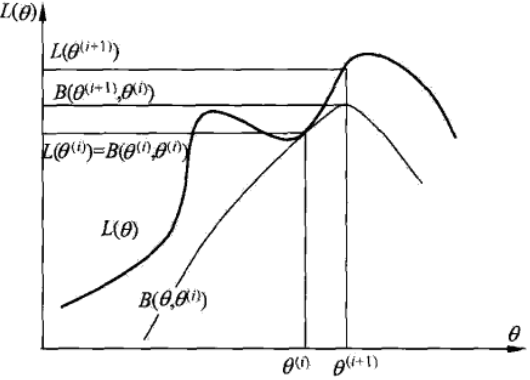
\includegraphics[scale=.50]{EM-algorithm.png}
\caption{Graphical interpretation of a single iteration of the EM algorithm: The function $B(\vec{\theta},\vec{\theta}^{t-1})$ is bounded above by the log likelihood function $\ell(\vec{\theta})$. The functions are equal at $\vec{\theta} = \vec{\theta}^{t-1}$. The EM algorithm chooses $\vec{\theta}^{t-1}$ as the value of $\vec{\theta}$ for which $B(\vec{\theta},\vec{\theta}^{t-1})$ is a maximum. Since $\ell(\vec{\theta}) \geq B(\vec{\theta},\vec{\theta}^{t-1})$ increasing $B(\vec{\theta},\vec{\theta}^{t-1})$ ensures that the value of the log likelihood function $\ell(\vec{\theta})$ is increased at each step.}
\label{fig:EM-algorithm} 
\end{figure}

Since the expected complete data log likelihood $Q$ is derived from $B(\vec{\theta},\vec{\theta}^{t-1})$ by dropping terms which are constant w.r.t. $\vec{\theta}$, so it is also a lower bound to a lower bound of $\ell(\vec{\theta})$.


\subsubsection{EM monotonically increases the observed data log likelihood}


\subsection{Generalization of EM Algorithm *}
EM algorithm can be interpreted as F function's maximization-maximization algorithm, based on this interpretation there are many variations and generalization, e.g., generalized EM Algorithm(GEM).


\subsubsection{F function's maximization-maximization algorithm}
\begin{definition}
Given the probability distribution of the hidden variable $Z$ is $\tilde{P}(Z)$, define \textbf{F function} as the following:
\begin{equation}
F(\tilde{P},\vec{\theta})=\mathbb{E}_{\tilde{P}}\left[\log{P(X,Z|\theta)}\right]+H(\tilde{P})
\end{equation}
Where $H(\tilde{P})=-\mathbb{E}_{\tilde{P}}\log\tilde{P}(Z)$, which is $\tilde{P}(Z)$'s entropy. Usually we assume that $P(X,Z|\theta)$ is continuous w.r.t. $\vec{\theta}$, therefore $F(\tilde{P},\vec{\theta})$ is continuous w.r.t. $\tilde{P}$ and $\vec{\theta}$.
\end{definition}

\begin{lemma}
\label{lemma:F-function}
For a fixed $\vec{\theta}$, there is only one distribution $\tilde{P}_{\theta}$ which maximizes $F(\tilde{P},\vec{\theta})$
\begin{equation}
\tilde{P}_{\theta}(Z)=P(Z|X, \vec{\theta})
\end{equation}
and $\tilde{P}_{\theta}$ is continuous w.r.t. $\vec{\theta}$.
\end{lemma}

\begin{proof}
Given a fixed $\vec{\theta}$, we can get $\tilde{P}_{\theta}$ which maximizes $F(\tilde{P},\vec{\theta})$. we construct the Lagrangian
\begin{equation}\begin{split}
\mathcal{L}(\tilde{P}, \vec{\theta}) & =\mathbb{E}_{\tilde{P}}\left[\log{P(X,Z|\theta)}\right]-\mathbb{E}_{\tilde{P}}\log\tilde{P}_{\theta}(Z) \\
                                     & \quad +\lambda\left[1-\sum\limits_Z{\tilde{P}(Z)}\right]
\end{split}\end{equation}

Take partial derivative with respect to $\tilde{P}_{\theta}(Z)$ then we get
\begin{equation}
\dfrac{\partial \mathcal{L}}{\partial{\tilde{P}_{\theta}(Z)}}=\log{P(X,Z|\theta)}-\log\tilde{P}_{\theta}(Z)-1-\lambda  \nonumber
\end{equation}

Let it equal to 0, we can get
\begin{equation}
\lambda=\log{P(X,Z|\theta)}-\log\tilde{P}_{\theta}(Z)-1 \nonumber
\end{equation}

Then we can derive that $\tilde{P}_{\theta}(Z)$ is proportional to $P(X,Z|\theta)$
\begin{eqnarray}
\dfrac{P(X,Z|\theta)}{\tilde{P}_{\theta}(Z)} &=& e^{1+\lambda} \nonumber \\
\Rightarrow \tilde{P}_{\theta}(Z) &=& \dfrac{P(X,Z|\vec{\theta})}{e^{1+\lambda}} \nonumber \\
\sum\limits_Z{\tilde{P}_{\theta}(Z)}=1 & \Rightarrow & \sum\limits_Z{\dfrac{P(X,Z|\vec{\theta})}{e^{1+\lambda}}}=1 \Rightarrow P(X|\vec{\theta})=e^{1+\lambda} \nonumber \\
\tilde{P}_{\theta}(Z) &=& \dfrac{P(X,Z|\vec{\theta})}{e^{1+\lambda}} = \dfrac{P(X,Z|\vec{\theta})}{P(X|\vec{\theta})}=P(Z|X, \vec{\theta}) \nonumber
\end{eqnarray}
\end{proof}

\begin{lemma}
If $\tilde{P}_{\theta}(Z)=P(Z|X, \vec{\theta})$, then
\begin{equation}
F(\tilde{P},\vec{\theta})=\log P(X|\vec{\theta})
\end{equation}
\end{lemma}

\begin{theorem}
One iteration of EM algorithm can be implemented as F function's maximization-maximization.

Assume $\vec{\theta}^{t-1}$ is the estimation of $\vec{\theta}$ in the $(t-1)$-th iteration, $\tilde{P}^{t-1}$ is the estimation of $\tilde{P}$ in the $(t-1)$-th iteration. Then in the $t$-th iteration two steps are:
\begin{enumerate}
\item for fixed $\vec{\theta}^{t-1}$, find $\tilde{P}^t$ that maximizes $F(\tilde{P},\vec{\theta}^{t-1})$;
\item for fixed $\tilde{P}^t$, find $\vec{\theta}^t$ that maximizes $F(\tilde{P}^t,\vec{\theta})$.
\end{enumerate}
\end{theorem}

\begin{proof}
(1) According to Lemma \ref{lemma:F-function}, we can get
\begin{equation}
\tilde{P}^t(Z)=P(Z|X, \vec{\theta}^{t-1}) \nonumber
\end{equation}

(2) According above, we can get
\begin{eqnarray}
F(\tilde{P}^t,\vec{\theta}) &=& \mathbb{E}_{\tilde{P}^t}\left[\log{P(X,Z|\theta)}\right]+H(\tilde{P}^t) \nonumber \\
    &=& \sum\limits_Z{P(Z|X,\vec{\theta}^{t-1})\log{P(X,Z|\theta)}}+H(\tilde{P}^t) \nonumber \\
	&=& Q(\vec{\theta}, \vec{\theta}^{t-1})+H(\tilde{P}^t)\nonumber
\end{eqnarray}

Then
\begin{equation}
\vec{\theta}^t=\arg\max\limits_{\theta}F(\tilde{P}^t,\vec{\theta})=\arg\max\limits_{\theta}Q(\vec{\theta}, \vec{\theta}^{t-1}) \nonumber
\end{equation}
\end{proof}


\subsubsection{The Generalized EM Algorithm(GEM)}
In the formulation of the EM algorithm described above, $\vec{\theta}^t$ was chosen as the value of $\vec{\theta}$ for which $Q(\vec{\theta}, \vec{\theta}^{t-1})$ was maximized. While this ensures the greatest increase in $\ell(\vec{\theta})$, it is however possible to relax the requirement of maximization to one of simply increasing $Q(\vec{\theta}, \vec{\theta}^{t-1})$ so that $Q(\vec{\theta}^t, \vec{\theta}^{t-1}) \geq Q(\vec{\theta}^{t-1}, \vec{\theta}^{t-1})$. This approach, to simply increase and not necessarily maximize $Q(\vec{\theta}^t, \vec{\theta}^{t-1})$ is known as the Generalized Expectation Maximization (GEM) algorithm and is often useful in cases where the maximization is difficult. The convergence of the GEM algorithm is similar to the EM algorithm.


\subsection{Online EM}


\subsection{Other EM variants *}


\section{Model selection for latent variable models}
\label{sec:Model-selection-for-LVM}
When using LVMs, we must specify the number of latent variables, which controls the model complexity. In particular, in the case of mixture models, we must specify $K$, the number of clusters. Choosing these parameters is an example of model selection. We discuss some approaches below.


\subsection{Model selection for probabilistic models}
The optimal Bayesian approach, discussed in Section \ref{sec:Bayesian-model-selection}, is to pick the model with the largest marginal likelihood, $K^*=\arg\max_k p(\mathcal{D}|k)$.

There are two problems with this. First, evaluating the marginal likelihood for LVMs is quite difficult. In practice, simple approximations, such as BIC, can be used (see e.g., (Fraley and Raftery 2002)). Alternatively, we can use the cross-validated likelihood as a performance measure, although this can be slow, since it requires fitting each model $F$ times, where Fis the number of CV folds.

The second issue is the need to search over a potentially large number of models. The usual approach is to perform exhaustive search over all candidate values ofK. However, sometimes we can set the model to its maximal size, and then rely on the power of the Bayesian Occam’s razor to “kill off” unwanted components. An example of this will be shown in Section TODO 21.6.1.6, when we discuss variational Bayes.

An alternative approach is to perform stochastic sampling in the space of models. Traditional approaches, such as (Green 1998, 2003; Lunn et al. 2009), are based on reversible jump MCMC, and use birth moves to propose new centers, and death moves to kill off old centers. However, this can be slow and difficult to implement. A simpler approach is to use a Dirichlet process mixture model, which can be fit using Gibbs sampling, but still allows for an unbounded number of mixture components; see Section TODO 25.2 for details.

Perhaps surprisingly, these sampling-based methods can be faster than the simple approach of evaluating the quality of eachKseparately. The reason is that fitting the model for each $K$ is often slow. By contrast, the sampling methods can often quickly determine that a certain value of $K$ is poor, and thus they need not waste time in that part of the posterior.


\subsection{Model selection for non-probabilistic methods}
What if we are not using a probabilistic model? For example, how do we choose $K$ for the K-means algorithm? Since this does not correspond to a probability model, there is no likelihood, so none of the methods described above can be used.

An obvious proxy for the likelihood is the \textbf{reconstruction error}. Define the squared reconstruction error of a data set $\mathcal{D}$, using model complexity $K$, as follows:
\begin{equation}
E(\mathcal{D}, K) \triangleq \frac{1}{|\mathcal{D}|}\sum\limits_{i=1}^N \lVert\vec{x}_i-\hat{\vec{x}}_i\rVert^2
\end{equation}

In the case of K-means, the reconstruction is given by $\hat{\vec{x}}_i=\vec{\mu}_{z_i}$, where $z_i=\arg\min_k \lVert\vec{x}_i-\hat{\vec{\mu}}_k\rVert^2$, as explained in Section 11.4.2.6 TODO.

In supervised learning, we can always use cross validation to select between non-probabilistic models of different complexity, but this is not the case with unsupervised learning. The most common approach is to plot the reconstruction error on the training set versus $K$, and to try to identify a \textbf{knee} or \textbf{kink} in the curve. 


\section{Fitting models with missing data}
Suppose we want to fit a joint density model by maximum likelihood, but we have “holes” in our data matrix, due to missing data (usually represented by NaNs). More formally, let $O_{ij} =1$ if component $j$ of data case $i$ is observed, and let $O_{ij} =0$ otherwise. Let $\vec{X}_v=\{x_{ij}: \vec{O}_{ij} =1\}$ be the visible data, and $X_h=\{x_{ij}: \vec{O}_{ij} =0\}$ be the missing or hidden data. Our goal is to compute
\begin{equation}
\hat{\vec{\theta}}=\arg\max_{\vec{\theta}} p(\vec{X}_v|\vec{\theta}, \vec{O})
\end{equation}

Under the missing at random assumption (see Section \ref{sec:Dealing-with-missing-data}), we have

TODO

\subsection{EM for the MLE of an MVN with missing data}
TODO
